
\section{Registers}

There are many registers in the x86 architecture, but we will only focus on the
ones necessary for learning basic Assembly and essential for future binary
exploitation.

\subsection{Intel 32 bites registers}


\subsubsection{General purpose registers}
\begin{itemize}
    \item \verb+EAX+ Extended Accumulator Register
    \item \verb+EBX+ Extended Base Register
    \item \verb+ECD+ Extended Counter Register
    \item \verb+EDX+ Extended Data Register
    \item \verb+ESI+ Extended Source Index
    \item \verb+EDI+ Extended Destination Index
    \item \verb+EBP+ Extended Base Pointer
    \item \verb+ESP+ Extended Stack Pointer
\end{itemize}

All the general purpose registers are 32-bit size in Intel’s IA-32 architecture but depending
on their origin and intended purpose, a subset of some of them can be referenced in
assembly.
\begin{verbatim}
32 bits         16 bits         8 bits
EAX             AX              AH / AL
EBX             BX              BH / BL
ECX             CX              CH / CL
EDX             DX              DH / DL
ESI             SI
EDI             DI
EBP             BP
ESP             SP
\end{verbatim}

\verb+AX+ to \verb+SP+ are the 16 bit registers used to reference the 16 least
significant bits in their equivalent 32 bit registers. The eight bit registers
reference the higher and lower eight bits of the 16 bit registers.

\subsubsection{Segment registers}
are used to make segmental distinctions in the binary. We will
approach segments later but in short, the hexadecimal value \verb+0x90+ can
either represent an instruction or a data value. The CPU knows which one thanks
to segment registe.

\subsubsection{Status flag registers}
Flags are tiny bit values that are either set (1)
or not set (0). Each flag represent a status. For example, if the “signed” flag
is set, the value of FF will represent a \verb+-1+ in decimal notation instead
of \verb+255+. Flags are all stored in special flag register, were many one bit
flags are stored at once. The flags are set whenever an operation resulted in
certain state or output. The flags we are most interested in for now are:
\begin{itemize}
        \item Z – zero flag, set when the result of the last operation is zero
            32 bits 16 bits 8 bit
        \item S – signed flag, set to determine if values should be intercepted
            as signed or unsigned
        \item O – overflow flag, set when the result of the last operation
            switches the most significant bit from either F to 0 or 0 to F.
        \item C – carry flag, set when the result of the last operation changes
            the most significant bit
\end{itemize}

{\bf Extended Instruction Pointer (EIP)} The instruction pointer has the same
function in a CPU as the needle had in those old gramophones your grandpa used
to have. It points to the next instruction to be executed.


\subsection{Intel 64 bites registers}


\subsubsection{General purpose registers} 

Sixteen general purpose 64-bit registers:
\begin{itemize}
        \item eight  RAX, RBX, RCX, RDX, RBP, RSI, RDI, and RSP. 
        \item eight are named R8-R15.
\end{itemize}

By replacing the initial \verb+R+ with an \verb+E+ on the first eight
registers, it is possible to access the lower 32 bits (\verb+EAX+ for
\verb+RAX+). 

Similarly, for \verb+RAX+, access to the lower 16 bits is possible by removing
the initial \verb+R+ , and the lower byte of the these by switching the
\verb+X+ for \verb+L+ (\verb+AL+ for \verb+AX+), and the higher byte of the low
16 bits using an \verb+H+ (\verb+AH+ for \verb+AX+). 

The new registers \verb+R8+ to \verb+R15+ can be accessed in a similar manner
like this: \verb+R8+ (qword), \verb+R8D+ (lower dword), \verb+R8W+ (lowest
word), \verb+R8B+ (lowest byte MASM style, Intel style \verb+R8L+). Note there
is no \verb+R8H+


 \begin{figure}
  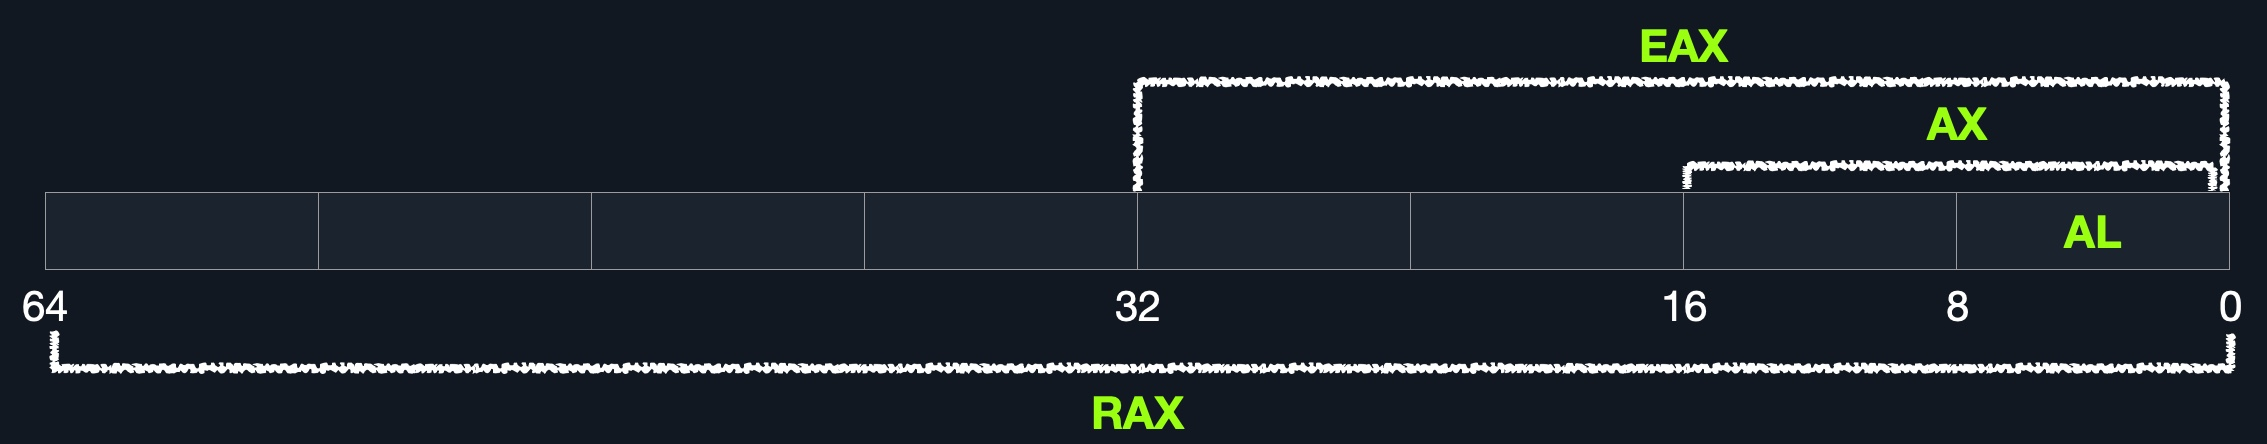
\includegraphics[width=\linewidth]{binary/archi/images/assembly_register_parts.jpg}
  \caption{Registry parts}
  \label{fig:assembly_register_parts}
\end{figure}

 \begin{figure}
  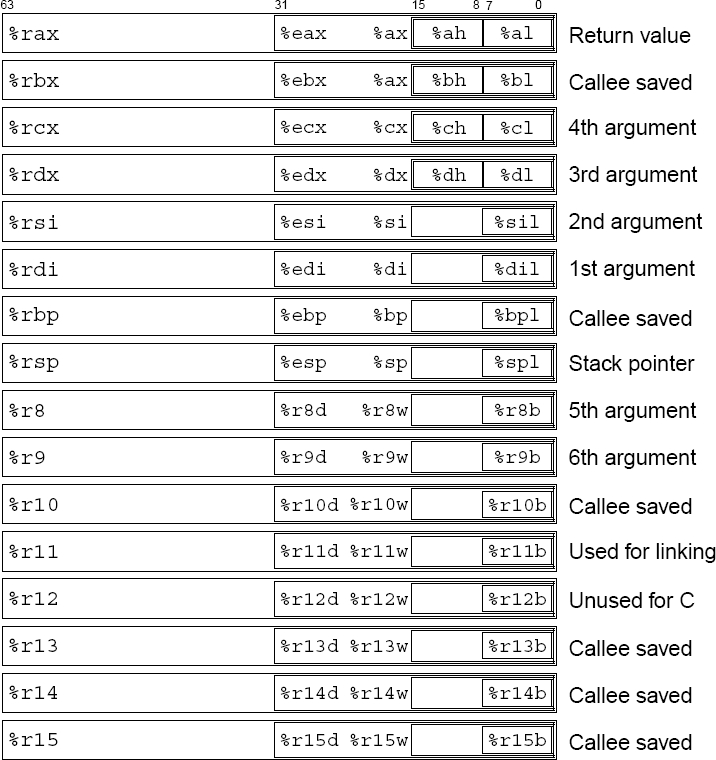
\includegraphics[width=\linewidth]{binary/archi/images/x86_64-registers.jpg}
  \caption{x86 64 general registers}
  \label{fig:ix86_64-registers}
\end{figure}

\begin{verbatim}
Data/Arguments Registers
    Syscall Number/Return value 	rax 
    Callee Saved 	                rbx 	
    1st arg - Destination operand 	rdi 	
    2nd arg - Source operand  	    rsi 	
    3rd arg 	                    rdx 	
    4th arg - Loop counter 	        rcx 	
    5th arg 	                    r8 	
    6th arg 	                    r9
Pointer Registers
    Base Stack Pointer 	            rbp
    Current/Top Stack Pointer 	    rsp 
    Instruction Pointer 'call only' rip
\end{verbatim}
